% Slide 3: Naive Bayes Introduction
\begin{frame}{طبقه‌بند بیز ساده}{\lr{Naïve Bayes Classifier}}
  \begin{itemize}
    \setlength{\itemsep}{7pt}
    \item یک روش طبقه‌بندی \textbf{احتمالاتی} مبتنی بر قضیه بیز (\lr{Bayes Theorem}).
    \begin{itemize}
      \item روشی کلاسیک و بسیار موفق در کاربردهای مختلف: پردازش زبان طبیعی (\lr{NLP})، سیستم‌های توصیه‌گر (\lr{Recommender Systems}) و فیلتر هرزنامه.
    \end{itemize}
    \item \textbf{هدف اصلی:} برآورد محتمل‌ترین برچسب کلاس برای یک نمونه یا رکورد ورودی داده‌شده.
    \item \textbf{فرمول‌بندی احتمالاتی مسئله طبقه‌بندی:}
    \begin{itemize}
      \item در نظر گرفتن هر ویژگی $A_i$ و برچسب کلاس $C$ به عنوان متغیرهای تصادفی.
      \item با داشتن بردار ویژگی‌های $(A_1, A_2, \dots, A_n)$، هدف یافتن کلاسی مانند $C$ است که احتمال شرطی زیر را بیشینه کند:
      \[
        \arg\max_C P(C \mid A_1, A_2, \dots, A_n)
      \]
    \end{itemize}
    \item \textbf{مثال کاربردی:} آیا امروز گلف بازی کنیم یا خیر؟
    \begin{itemize}
      \item $P(\text{Play}=\text{yes} \mid \text{Outlook}=\text{rainy}, \text{Temp}=\text{cool})$
      \item $P(\text{Play}=\text{no} \mid \text{Outlook}=\text{rainy}, \text{Temp}=\text{cool})$
    \end{itemize}
  \end{itemize}
\end{frame}

% Slide 4: Thomas Bayes & Bayes Theorem
\begin{frame}{تاریخچه طبقه‌بند بیز}{\lr{Thomas Bayes (1701--1761)}}
  \begin{columns}[T]
    \begin{column}{0.64\textwidth}
      \begin{itemize}
        \setlength{\itemsep}{10pt}
        \item \textbf{توماس بیز:} \lr{(Thomas Bayes)}
        \begin{itemize}
          \setlength{\itemsep}{4pt}
          \item ریاضی‌دان و کشیش بریتانیایی.
          \item تلاش برای اثبات صوری و ریاضیاتی وجود خداوند با استفاده از محاسبات احتمالات.
        \end{itemize}
        \item \textbf{قضیه بیز:} \lr{(Bayes Theorem)}
        \begin{itemize}
          \setlength{\itemsep}{4pt}
          \item یکی از مهم‌ترین و بنیادی‌ترین قضایای نظریه احتمالات و آمار کاربردی.
          \item این نظریه برجسته تنها پس از درگذشت وی در سال ۱۷۶۳ توسط ریچارد پرایس منتشر گردید.
        \end{itemize}
      \end{itemize}
    \end{column}
    \begin{column}{0.34\textwidth}
      \begin{center}
        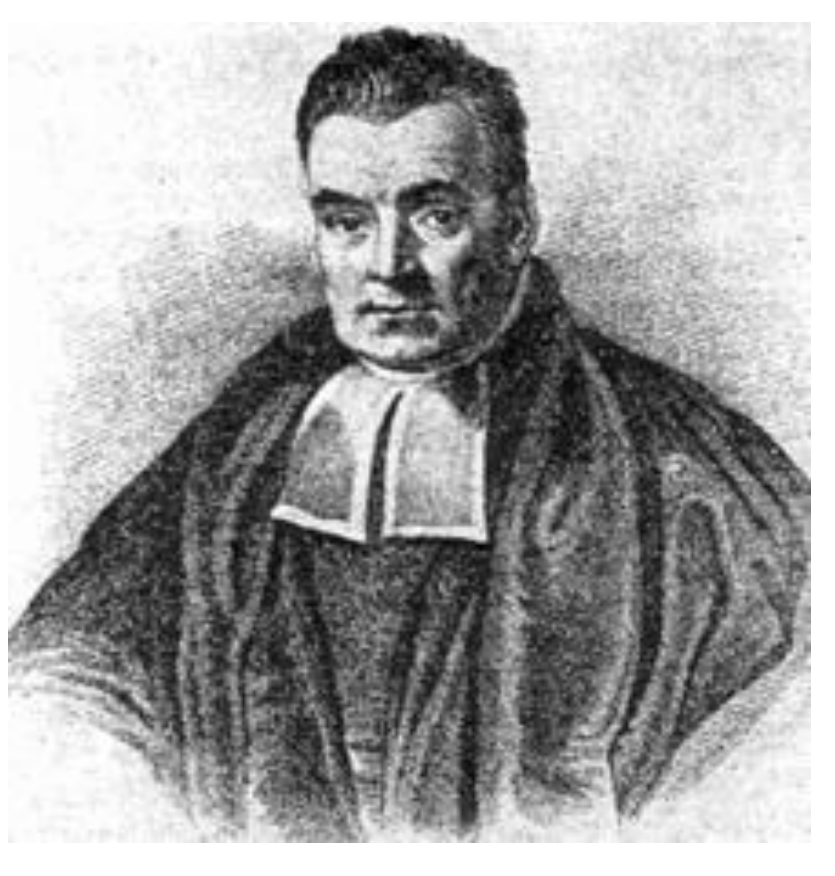
\includegraphics[width=0.88\textwidth,height=4.5cm,keepaspectratio]{images/slide04_thomas_bayes.png}\\[0.15cm]
        {\fontsize{7.5}{9}\selectfont\color{subgray}توماس بیز (۱۷۰۱--۱۷۶۱)}
      \end{center}
    \end{column}
  \end{columns}
\end{frame}

% Slide 5: Bayes Theorem Formulation
\begin{frame}{فرمول‌بندی قضیه بیز}{\lr{Bayes Theorem Formulation}}
  \begin{itemize}
    \setlength{\itemsep}{8pt}
    \item \textbf{پرسش اساسی:} با مشاهده مجموعه ویژگی‌های $A$، احتمال تعلق به کلاس $C$ چقدر است؟
    \begin{itemize}
      \item این کمیت را \textbf{احتمال شرطی} یا احتمال پسین (\lr{Posterior Probability}) می‌نامیم: $P(C \mid A)$.
    \end{itemize}
    \item \textbf{سازوکار قضیه بیز:}
    \begin{itemize}
      \item قضیه بیز احتمال شرطی $P(C \mid A)$ را با استفاده از احتمال معکوس آن $P(A \mid C)$ و احتمالات پایه‌ای $P(A)$ و $P(C)$ محاسبه می‌کند:
    \end{itemize}
  \end{itemize}
  \vspace{0.2cm}
  \begin{center}
    \colorbox{codebg}{%
      \fontsize{13}{16}\selectfont
      $P(C \mid A) = \dfrac{P(A \mid C) \cdot P(C)}{P(A)}$
    }
  \end{center}
  \vspace{0.2cm}
  \begin{itemize}
    \item \textbf{کاربرد کلیدی:} زمانی که $P(C \mid A)$ مستقیماً در دسترس نیست، اما برآورد $P(A \mid C)$ (درست‌نمایی یا \lr{Likelihood}) و $P(C)$ از داده‌های آموزشی بسیار آسان است.
  \end{itemize}
\end{frame}

% Slide 6: Prior vs Posterior Probability
\begin{frame}{احتمال پیشین در برابر احتمال پسین}{\lr{Prior vs. Posterior Probability}}
  \begin{itemize}
    \setlength{\itemsep}{10pt}
    \item \textbf{\textcolor{mannheimteal}{احتمال پیشین}} برای کلاس $C$ \lr{($P(C)$ -- Prior Probability)}:
    \begin{itemize}
      \setlength{\itemsep}{4pt}
      \item احتمال وقوع کلاس $C$ پیش از مشاهده ویژگی‌ها یا شواهد $A$.
      \item به عنوان مثال، اگر در \lr{70\%} تمام موارد گلف بازی کرده باشیم:
      \[
        P(\text{Play}=\text{yes}) = 0.7
      \]
    \end{itemize}
    \item \textbf{\textcolor{mannheimblue}{احتمال پسین}} برای کلاس $C$ \lr{($P(C \mid A)$ -- Posterior Probability)}:
    \begin{itemize}
      \setlength{\itemsep}{4pt}
      \item احتمال تعلق به کلاس $C$ پس از مشاهده ویژگی‌های $A$ (شواهد).
      \item به عنوان مثال، اگر هوا بارانی و همراه با باد شدید باشد:
      \[
        P(\text{Play}=\text{yes} \mid A) = 0.2
      \]
    \end{itemize}
  \end{itemize}
\end{frame}

% Slide 7: Estimating Prior Probability
\begin{frame}{برآورد احتمال پیشین}{\lr{Estimating the Prior Probability $P(C)$}}
  \begin{itemize}
    \setlength{\itemsep}{10pt}
    \item احتمال پیشین $P(C_j)$ به سادگی از طریق \textbf{فراوانی نسبی} هر کلاس در کل داده‌های آموزشی برآورد می‌شود:
    \[
      P(C_j) = \frac{|D_{C_j}|}{|D|}
    \]
    \item در این رابطه:
    \begin{itemize}
      \setlength{\itemsep}{4pt}
      \item $|D_{C_j}|$ برابر است با تعداد کل رکوردهای متعلق به کلاس $C_j$ در مجموعه آموزش.
      \item $|D|$ برابر است با تعداد کل رکوردهای آموزشی.
    \end{itemize}
    \item \textbf{مثال بازی گلف} (مجموع داده‌های ۱۴ روز):
    \begin{itemize}
      \item تعداد روزهای با پاسخ مثبت: ۹ روز $\implies P(\text{Play}=\text{yes}) = \dfrac{9}{14} \approx 0.643$
      \item تعداد روزهای با پاسخ منفی: ۵ روز $\implies P(\text{Play}=\text{no}) = \dfrac{5}{14} \approx 0.357$
    \end{itemize}
  \end{itemize}
\end{frame}

% Slide 8: Estimating Class-Conditional Probability
\begin{frame}{برآورد درست‌نمایی شرطی کلاس}{\lr{Class-Conditional Probability $P(A \mid C)$}}
  \begin{itemize}
    \setlength{\itemsep}{8pt}
    \item \textbf{فرض بنیادین بیز «ساده»} (\lr{Conditional Independence Assumption}):
    \begin{itemize}
      \item فرض می‌شود تمام ویژگی‌های $A_1, A_2, \dots, A_n$ به شرط داشتن کلاس $C$، \textbf{از یکدیگر از نظر آماری مستقل هستند}.
    \end{itemize}
    \item بر این اساس، احتمال توأم به حاصل‌ضرب احتمالات شرطی تک‌تک ویژگی‌ها تبدیل می‌شود:
    \[
      P(A \mid C_j) = P(A_1, A_2, \dots, A_n \mid C_j) = \prod_{i=1}^{n} P(A_i \mid C_j)
    \]
    \item \textbf{مزیت بزرگ این فرض:}
    \begin{itemize}
      \item به جای برآورد توزیع توأم چندمتغیره پیچیده، کافی است احتمال هر ویژگی منفرد را به تفکیک هر کلاس محاسبه کنیم:
      \[
        P(A_i \mid C_j) = \frac{N_{i,j}}{|D_{C_j}|}
      \]
    \end{itemize}
  \end{itemize}
\end{frame}

% Slide 9: Weather Dataset Probabilities
\begin{frame}{محاسبه احتمالات در مجموعه داده آب‌وهوا}{\lr{Weather Dataset Frequency Tables}}
  \centering
  \scriptsize
  \setlength{\tabcolsep}{3pt}
  \begin{columns}[T]
    \begin{column}{0.44\textwidth}
      \textbf{جدول داده‌های آموزش (۱۴ رکورد)}\\[0.1cm]
      \begin{latin}
      \begin{tabular}{|c|c|c|c|c|}
        \hline
        \textbf{Outlook} & \textbf{Temp} & \textbf{Humidity} & \textbf{Windy} & \textbf{Play} \\
        \hline
        Sunny & Hot & High & False & No \\
        Sunny & Hot & High & True & No \\
        Overcast & Hot & High & False & Yes \\
        Rainy & Mild & High & False & Yes \\
        Rainy & Cool & Normal & False & Yes \\
        Rainy & Cool & Normal & True & No \\
        Overcast & Cool & Normal & True & Yes \\
        Sunny & Mild & High & False & No \\
        Sunny & Cool & Normal & False & Yes \\
        Rainy & Mild & Normal & False & Yes \\
        Sunny & Mild & Normal & True & Yes \\
        Overcast & Mild & High & True & Yes \\
        Overcast & Hot & Normal & False & Yes \\
        Rainy & Mild & High & True & No \\
        \hline
      \end{tabular}
      \end{latin}
    \end{column}
    \begin{column}{0.54\textwidth}
      \textbf{جداول فراوانی شرطی و احتمالات:}\\[0.1cm]
      \begin{latin}
      \begin{tabular}{|l|cc|cc|}
        \hline
        \multirow{2}{*}{\textbf{Attribute}} & \multicolumn{2}{c|}{\textbf{Counts}} & \multicolumn{2}{c|}{\textbf{Conditional Prob.}} \\
        & Yes & No & $P(A_i|\text{Yes})$ & $P(A_i|\text{No})$ \\
        \hline
        \multicolumn{5}{|l|}{\textbf{Outlook}} \\
        Sunny & 2 & 3 & $2/9$ & $3/5$ \\
        Overcast & 4 & 0 & $4/9$ & $0/5$ \\
        Rainy & 3 & 2 & $3/9$ & $2/5$ \\
        \hline
        \multicolumn{5}{|l|}{\textbf{Temperature}} \\
        Hot & 2 & 2 & $2/9$ & $2/5$ \\
        Mild & 4 & 2 & $4/9$ & $2/5$ \\
        Cool & 3 & 1 & $3/9$ & $1/5$ \\
        \hline
        \multicolumn{5}{|l|}{\textbf{Humidity}} \\
        High & 3 & 4 & $3/9$ & $4/5$ \\
        Normal & 6 & 1 & $6/9$ & $1/5$ \\
        \hline
        \multicolumn{5}{|l|}{\textbf{Windy}} \\
        False & 6 & 2 & $6/9$ & $2/5$ \\
        True & 3 & 3 & $3/9$ & $3/5$ \\
        \hline
      \end{tabular}
      \end{latin}
    \end{column}
  \end{columns}
\end{frame}

% Slide 10: Classifying a New Record - Concept
\begin{frame}{طبقه‌بندی یک رکورد جدید}{\lr{Classifying an Unseen Record}}
  \begin{itemize}
    \item فرض کنید رکورد جدیدی با مشخصات زیر وارد سیستم شده است:
  \end{itemize}
  \vspace{-0.1cm}
  \begin{center}
    \small
    \begin{latin}
    \begin{tabular}{|c|c|c|c|c|}
      \hline
      \textbf{Outlook} & \textbf{Temp.} & \textbf{Humidity} & \textbf{Windy} & \textbf{Play} \\
      \hline
      Sunny & Cool & High & True & \textbf{?} \\
      \hline
    \end{tabular}
    \end{latin}
  \end{center}
  \vspace{0.1cm}
  \begin{itemize}
    \item \textbf{محاسبه احتمال پسین برای کلاس \lr{Play = Yes} به صورت زیر است:}
  \end{itemize}
  \vspace{-0.1cm}
  {\small
  \[
    P(\text{yes} \mid A) = \frac{P(\text{Sunny}|\text{yes}) \cdot P(\text{Cool}|\text{yes}) \cdot P(\text{High}|\text{yes}) \cdot P(\text{True}|\text{yes}) \cdot P(\text{yes})}{P(A)}
  \]}
  \[
    P(\text{yes} \mid A) = \frac{\frac{2}{9} \times \frac{3}{9} \times \frac{3}{9} \times \frac{3}{9} \times \frac{9}{14}}{P(A)}
  \]
  \begin{itemize}
    \item مخرج کسر ($P(A)$) برای هر دو کلاس یکسان است و به عنوان ضریب نرمال‌سازی عمل می‌کند.
  \end{itemize}
\end{frame}

% Slide 11: Classifying a New Record - Comparison
\begin{frame}{محاسبه درست‌نمایی و نرمال‌سازی}{انتخاب کلاس برنده}
  \begin{itemize}
    \setlength{\itemsep}{5pt}
    \item \textbf{درست‌نمایی کلاس‌های دوگانه (\lr{Likelihood})}
    \begin{align*}
      \text{Likelihood}(\text{yes}) &= \frac{2}{9} \times \frac{3}{9} \times \frac{3}{9} \times \frac{3}{9} \times \frac{9}{14} = 0.0053 \\[4pt]
      \text{Likelihood}(\text{no})  &= \frac{3}{5} \times \frac{1}{5} \times \frac{4}{5} \times \frac{3}{5} \times \frac{5}{14} = 0.0206
    \end{align*}
    \item \textbf{تبدیل به احتمالات استاندارد با نرمال‌سازی (\lr{Normalization})}
    \begin{align*}
      P(\text{yes}) &= \frac{0.0053}{0.0053 + 0.0206} = 0.205 \quad (20.5\%) \\[4pt]
      P(\text{no})  &= \frac{0.0206}{0.0053 + 0.0206} = 0.795 \quad (79.5\%)
    \end{align*}
    \item \textbf{تصمیم نهایی:} از آنجا که $P(\text{no}) > P(\text{yes})$، برچسب پیش‌بینی‌شده برای این روز \textbf{\lr{Play = No}} خواهد بود.
  \end{itemize}
\end{frame}

% Slide 12: Handling Numerical Attributes - Options
\begin{frame}{مدیریت ویژگی‌های عددی و پیوسته}{\lr{Handling Numerical Attributes}}
  \begin{columns}[T]
    \begin{column}{0.56\textwidth}
      \begin{itemize}
        \setlength{\itemsep}{8pt}
        \item \textbf{رویکرد اول: گسسته‌سازی (\lr{Discretization})}
        \begin{itemize}
          \item تبدیل مقادیر پیوسته به بازه‌ها پیش از یادگیری طبقه‌بند.
          \item به عنوان مثال: \lr{Temp = 37$^\circ$C $\to$ "Hot"} و \lr{Temp = 21$^\circ$C $\to$ "Mild"}.
        \end{itemize}
        \item \textbf{رویکرد دوم: فرض توزیع نرمال گوسی}
        \begin{itemize}
          \item فرض می‌شود ویژگی عددی به شرط کلاس از \textbf{توزیع نرمال} پیروی می‌کند.
          \item برآورد میانگین ($\mu$) و انحراف معیار ($\sigma$) از روی نمونه‌های آموزشی هر کلاس.
          \item محاسبه $P(A_i \mid C_j)$ با تابع چگالی احتمال (\lr{PDF}).
        \end{itemize}
      \end{itemize}
    \end{column}
    \begin{column}{0.42\textwidth}
      \begin{center}
        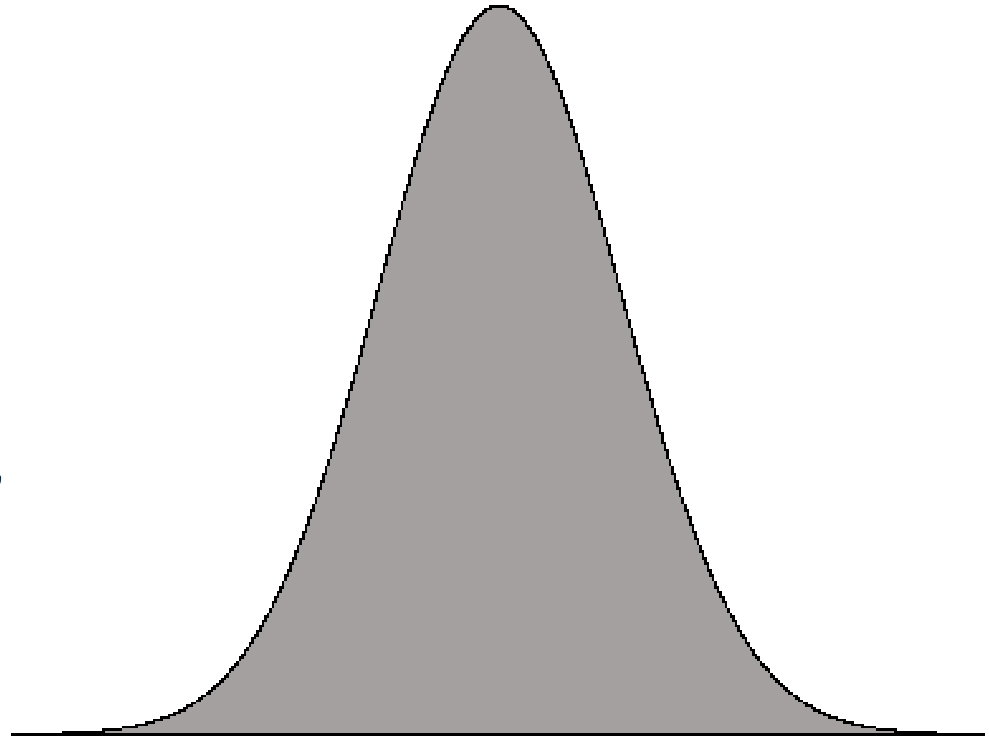
\includegraphics[width=\textwidth,height=4.2cm,keepaspectratio]{images/slide12_normal_dist.png}\\[0.1cm]
        {\fontsize{7.5}{9}\selectfont\color{subgray}منحنی چگالی توزیع نرمال گوسی}
      \end{center}
    \end{column}
  \end{columns}
\end{frame}

% Slide 13: Normal Distribution PDF Formula
\begin{frame}{تابع چگالی احتمال توزیع نرمال}{\lr{Gaussian Probability Density Function}}
  \begin{itemize}
    \setlength{\itemsep}{6pt}
    \item تابع چگالی احتمال (\lr{PDF}) برای متغیر پیوسته $x$ با توزیع نرمال:
    \[
      f(x) = \frac{1}{\sqrt{2\pi}\sigma} \exp\left(-\frac{(x - \mu)^2}{2\sigma^2}\right)
    \]
    \item پارامترهای توزیع که از داده‌های آموزشی برآورد می‌شوند:
    \begin{itemize}
      \item \textbf{میانگین نمونه} ($\mu$):
      \[
        \mu = \frac{1}{n} \sum_{i=1}^{n} x_i
      \]
      \item \textbf{انحراف معیار نمونه} ($\sigma$):
      \[
        \sigma = \sqrt{\frac{1}{n-1}\sum_{i=1}^{n} (x_i - \mu)^2}
      \]
      \item هر دو پارامتر به طور مستقیم از روی داده‌های آموزش برآورد می‌گردند.
    \end{itemize}
  \end{itemize}
\end{frame}

% Slide 14: Numerical Attributes - Example Calculation
\begin{frame}{محاسبه پارامترهای گوسی در داده‌های آب‌وهوا}{برآورد $\mu$ و $\sigma$ برای دما و رطوبت}
  \begin{itemize}
    \item محاسبه میانگین و انحراف معیار برای ویژگی‌های عددی به تفکیک کلاس:
  \end{itemize}
  \begin{center}
    \small
    \begin{latin}
    \begin{tabular}{|l|cc|cc|}
      \hline
      \textbf{Attribute} & $\mu (\text{Yes})$ & $\sigma (\text{Yes})$ & $\mu (\text{No})$ & $\sigma (\text{No})$ \\
      \hline
      Temperature & $73.0$ & $6.2$ & $74.6$ & $7.9$ \\
      Humidity & $79.1$ & $10.2$ & $86.2$ & $9.7$ \\
      \hline
    \end{tabular}
    \end{latin}
  \end{center}
  \vspace{0.2cm}
  \begin{itemize}
    \item \textbf{نمونه محاسبه چگالی احتمال شرطی} برای دمای ۶۶ درجه در کلاس \lr{Yes} به صورت زیر است:
    \[
      f(\text{Temp}=66 \mid \text{yes}) = \frac{1}{\sqrt{2\pi} \cdot 6.2} \exp\left(-\frac{(66 - 73)^2}{2 \cdot (6.2)^2}\right) \approx 0.0340
    \]
    \item مقدار چگالی به عنوان جانشین احتمال شرطی در فرمول بیز قرار می‌گیرد.
  \end{itemize}
\end{frame}

% Slide 15: Classifying Day with Numerical Features
\begin{frame}{طبقه‌بندی روز جدید با ویژگی‌های پیوسته}{اعمال توابع چگالی گوسی}
  \begin{itemize}
    \item رکورد جدید با ویژگی‌های اسمی و عددی:
  \end{itemize}
  \vspace{-0.1cm}
  \begin{center}
    \small
    \begin{latin}
    \begin{tabular}{|c|c|c|c|c|}
      \hline
      \textbf{Outlook} & \textbf{Temp.} & \textbf{Humidity} & \textbf{Windy} & \textbf{Play} \\
      \hline
      Sunny & 66 & 90 & True & \textbf{?} \\
      \hline
    \end{tabular}
    \end{latin}
  \end{center}
  \vspace{0.1cm}
  \begin{itemize}
    \item \textbf{محاسبه درست‌نمایی با استفاده از چگالی‌های گوسی:}
    \begin{align*}
      \text{Likelihood}(\text{yes}) &= \frac{2}{9} \times 0.0340 \times 0.0221 \times \frac{3}{9} \times \frac{9}{14} = 0.000036 \\[3pt]
      \text{Likelihood}(\text{no})  &= \frac{3}{5} \times 0.0291 \times 0.0380 \times \frac{3}{5} \times \frac{5}{14} = 0.000136
    \end{align*}
    \item \textbf{احتمالات پسین پس از نرمال‌سازی:}
    \[
      P(\text{yes}) = \frac{0.000036}{0.000036 + 0.000136} \approx 20.9\%, \quad P(\text{no}) \approx 79.1\%
    \]
    \item \textbf{نکته کلیدی:} در صورت غیرنرمال بودن داده‌ها، باید از توزیع دیگری استفاده کرد یا داده را گسسته‌سازی نمود.
  \end{itemize}
\end{frame}

% Slide 16: Handling Missing Values
\begin{frame}{مدیریت داده‌های مفقوده}{\lr{Handling Missing Values in Naïve Bayes}}
  \begin{itemize}
    \setlength{\itemsep}{8pt}
    \item مقادیر مفقوده ممکن است در نمونه‌های آموزش یا نمونه‌های آزمون رخ دهند:
    \begin{itemize}
      \item \textbf{در زمان آموزش} (\lr{Training}): نمونه مفقود در شمارش فراوانی آن ویژگی لحاظ نمی‌شود، اما برای سایر ویژگی‌های موجود استفاده می‌گردد.
      \item \textbf{در زمان طبقه‌بندی} (\lr{Classification}): ویژگی مفقود از ضرب احتمالات شرطی کنار گذاشته می‌شود.
    \end{itemize}
    \item \textbf{مثال: رکورد آزمون با ویژگی دمای نامشخص (\lr{Temp = ?})}
    \begin{align*}
      \text{Likelihood}(\text{yes}) &= \frac{3}{9} \times \frac{3}{9} \times \frac{3}{9} \times \frac{9}{14} = 0.0238 \\[3pt]
      \text{Likelihood}(\text{no})  &= \frac{1}{5} \times \frac{4}{5} \times \frac{3}{5} \times \frac{5}{14} = 0.0343
    \end{align*}
    \item احتمالات پسین نرمال‌شده: \lr{$P(\text{yes}) = 41\%$} و \lr{$P(\text{no}) = 59\%$}.
  \end{itemize}
\end{frame}

% Slide 17: Zero-Frequency Problem & Laplace Smoothing
\begin{frame}{مسئله بسامد صفر و هموارسازی لاپلاس}{\lr{Zero-Frequency Problem \& Laplace Estimator}}
  \begin{itemize}
    \setlength{\itemsep}{6pt}
    \item \textbf{صورت مسئله:} اگر یک مقدار ویژگی در یک کلاس هرگز رخ نداده باشد:
    \begin{itemize}
      \item مثلاً در داده‌های آموزش: $P(\text{Outlook}=\text{Overcast} \mid \text{no}) = \frac{0}{5} = 0$.
      \item در نتیجه، کل حاصل‌ضرب درست‌نمایی صفر خواهد شد: \lr{$P(\text{no} \mid A) = 0$}.
    \end{itemize}
    \item \textbf{راه‌حل: برآوردگر لاپلاس (\lr{Laplace Estimator})}
    \begin{itemize}
      \item افزودن مقدار ثابت ۱ به صورت و مقدار $c$ (تعداد حالات ممکن ویژگی $A$) به مخرج کسر:
    \end{itemize}
  \end{itemize}
  \vspace{0.2cm}
  \begin{columns}[T]
    \begin{column}{0.44\textwidth}
      \textbf{برآورد احتمال استاندارد:}
      \[
        P(A_i \mid C) = \frac{N_{ic}}{N_c}
      \]
    \end{column}
    \begin{column}{0.44\textwidth}
      \textbf{برآوردگر هموارسازی لاپلاس:}
      \[
        P(A_i \mid C) = \frac{N_{ic} + 1}{N_c + c}
      \]
    \end{column}
  \end{columns}
  \vspace{0.2cm}
  \begin{itemize}
    \item \textbf{مزیت:} احتمال هیچ حالتی دقیقاً صفر نمی‌شود و تخمین پایدار می‌گردد.
  \end{itemize}
\end{frame}

% Slide 18: Conditional Probabilities & Python Implementation
\begin{frame}{اطمینان مدل و پیاده‌سازی پایتون}{\lr{Confidence \& Scikit-learn Implementation}}
  \begin{center}
    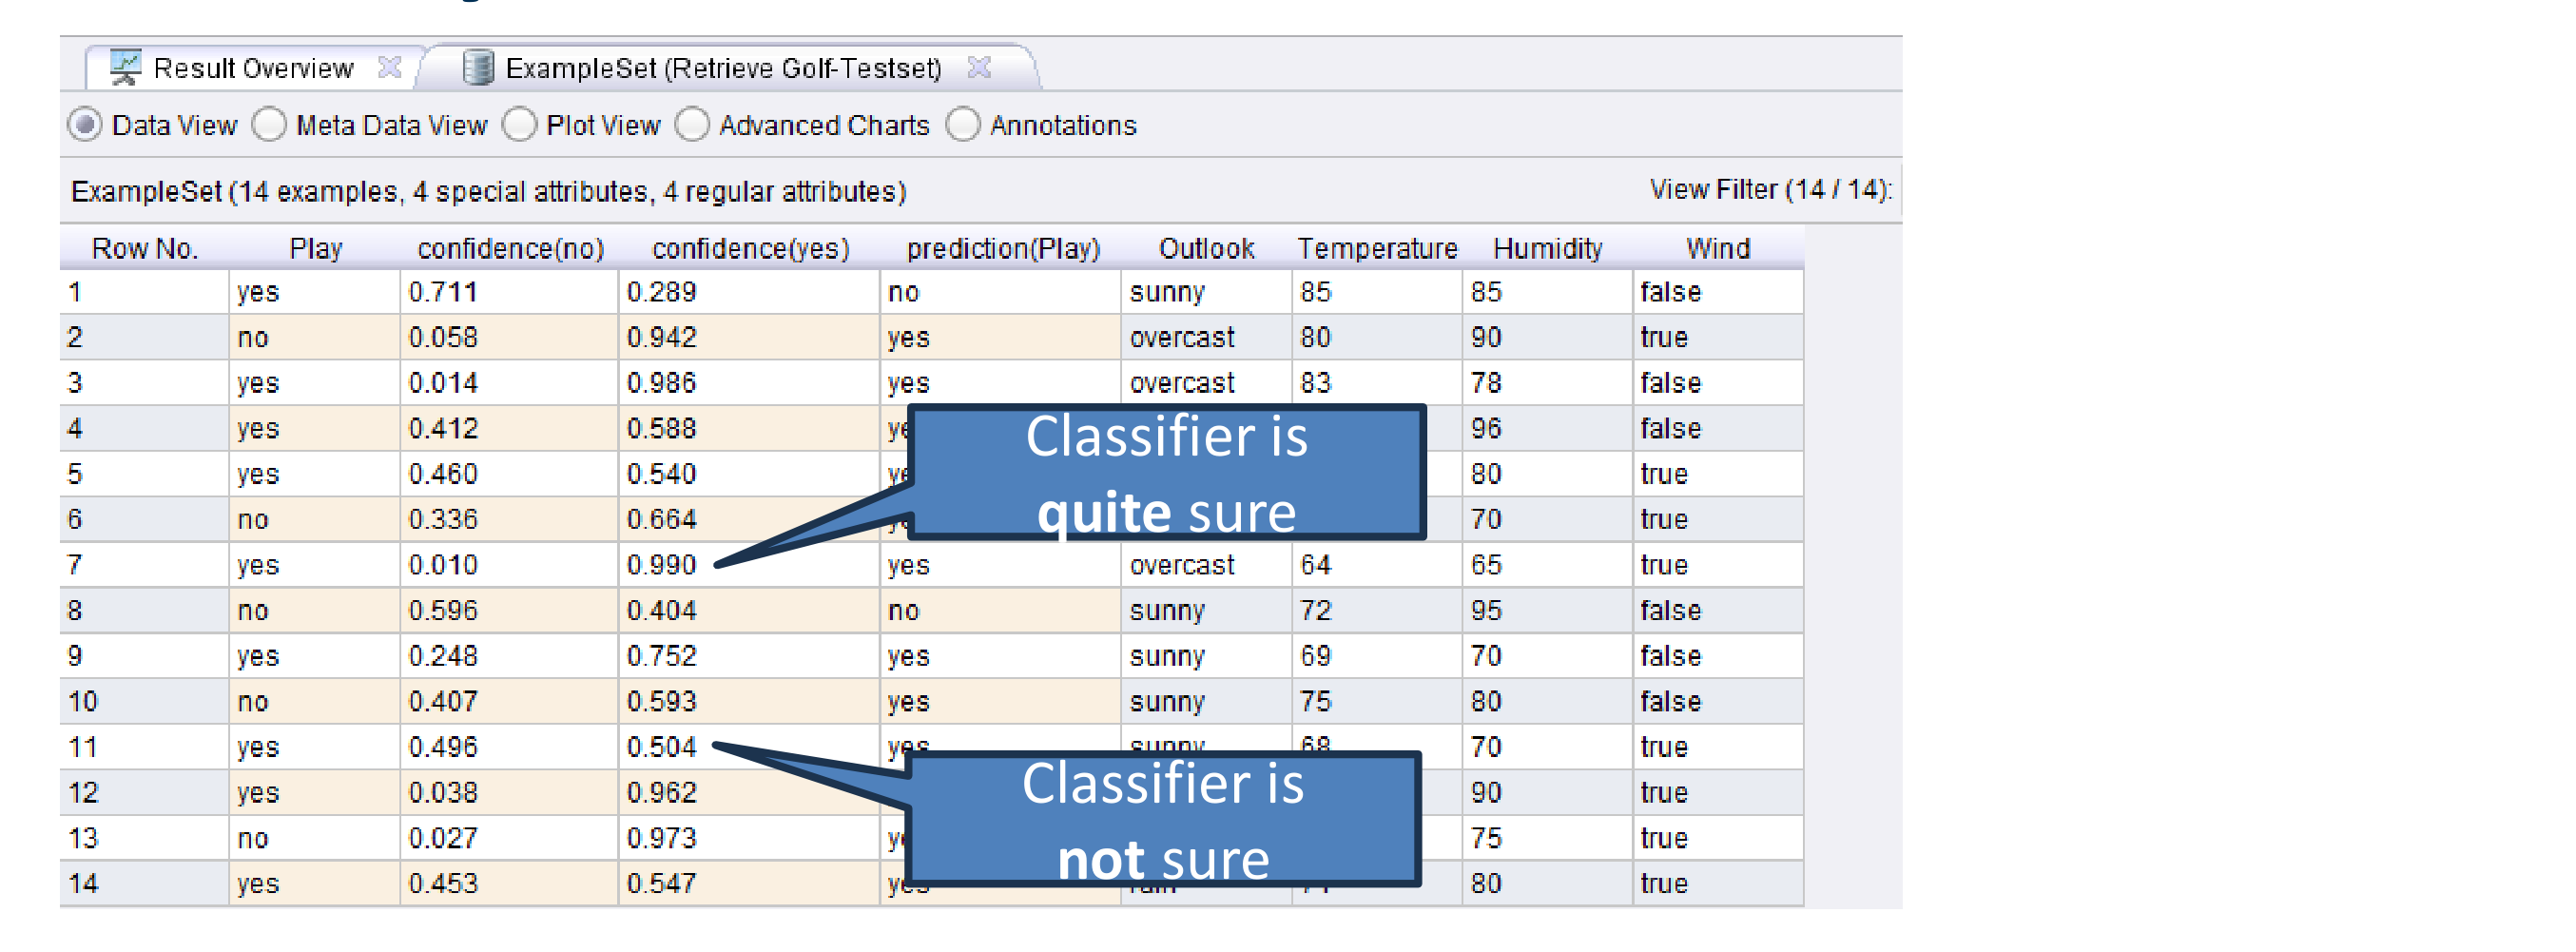
\includegraphics[width=0.92\textwidth,height=2.5cm,keepaspectratio]{images/slide18_table_callouts_clean.png}
  \end{center}
  \vspace{0.05cm}
  \begin{latin}
    \begin{minipage}{0.96\textwidth}
      \fcolorbox{codeborder}{codebg}{%
        \begin{minipage}{0.97\textwidth}
          \ttfamily\small
          \textcolor{mannheimteal}{\# Import Naive Bayes classifiers from scikit-learn}\\
          \textbf{from} sklearn.naive\_bayes \textbf{import} MultinomialNB, GaussianNB\\[4pt]
          \textcolor{mannheimteal}{\# Train classifier with Laplace smoothing (alpha=1.0)}\\
          estimator = MultinomialNB(alpha=1.0)\\
          estimator.fit(preprocessed\_training\_data, training\_labels)
        \end{minipage}%
      }
    \end{minipage}
  \end{latin}
\end{frame}

% Slide 19: Decision Boundaries of Naive Bayes
\begin{frame}{مرزهای تصمیم طبقه‌بند بیز ساده}{\lr{Decision Boundary of Naive Bayes Classifier}}
  \begin{itemize}
    \setlength{\itemsep}{8pt}
    \item نواحی منسجم و معمولاً بزرگ‌تر
    \item حاشیه‌ها و مرزهای نرم با نواحی عدم قطعیت
    \item شکل‌های دلخواه (اغلب به صورت منحنی)
  \end{itemize}
  \vspace{0.05cm}
  \begin{center}
    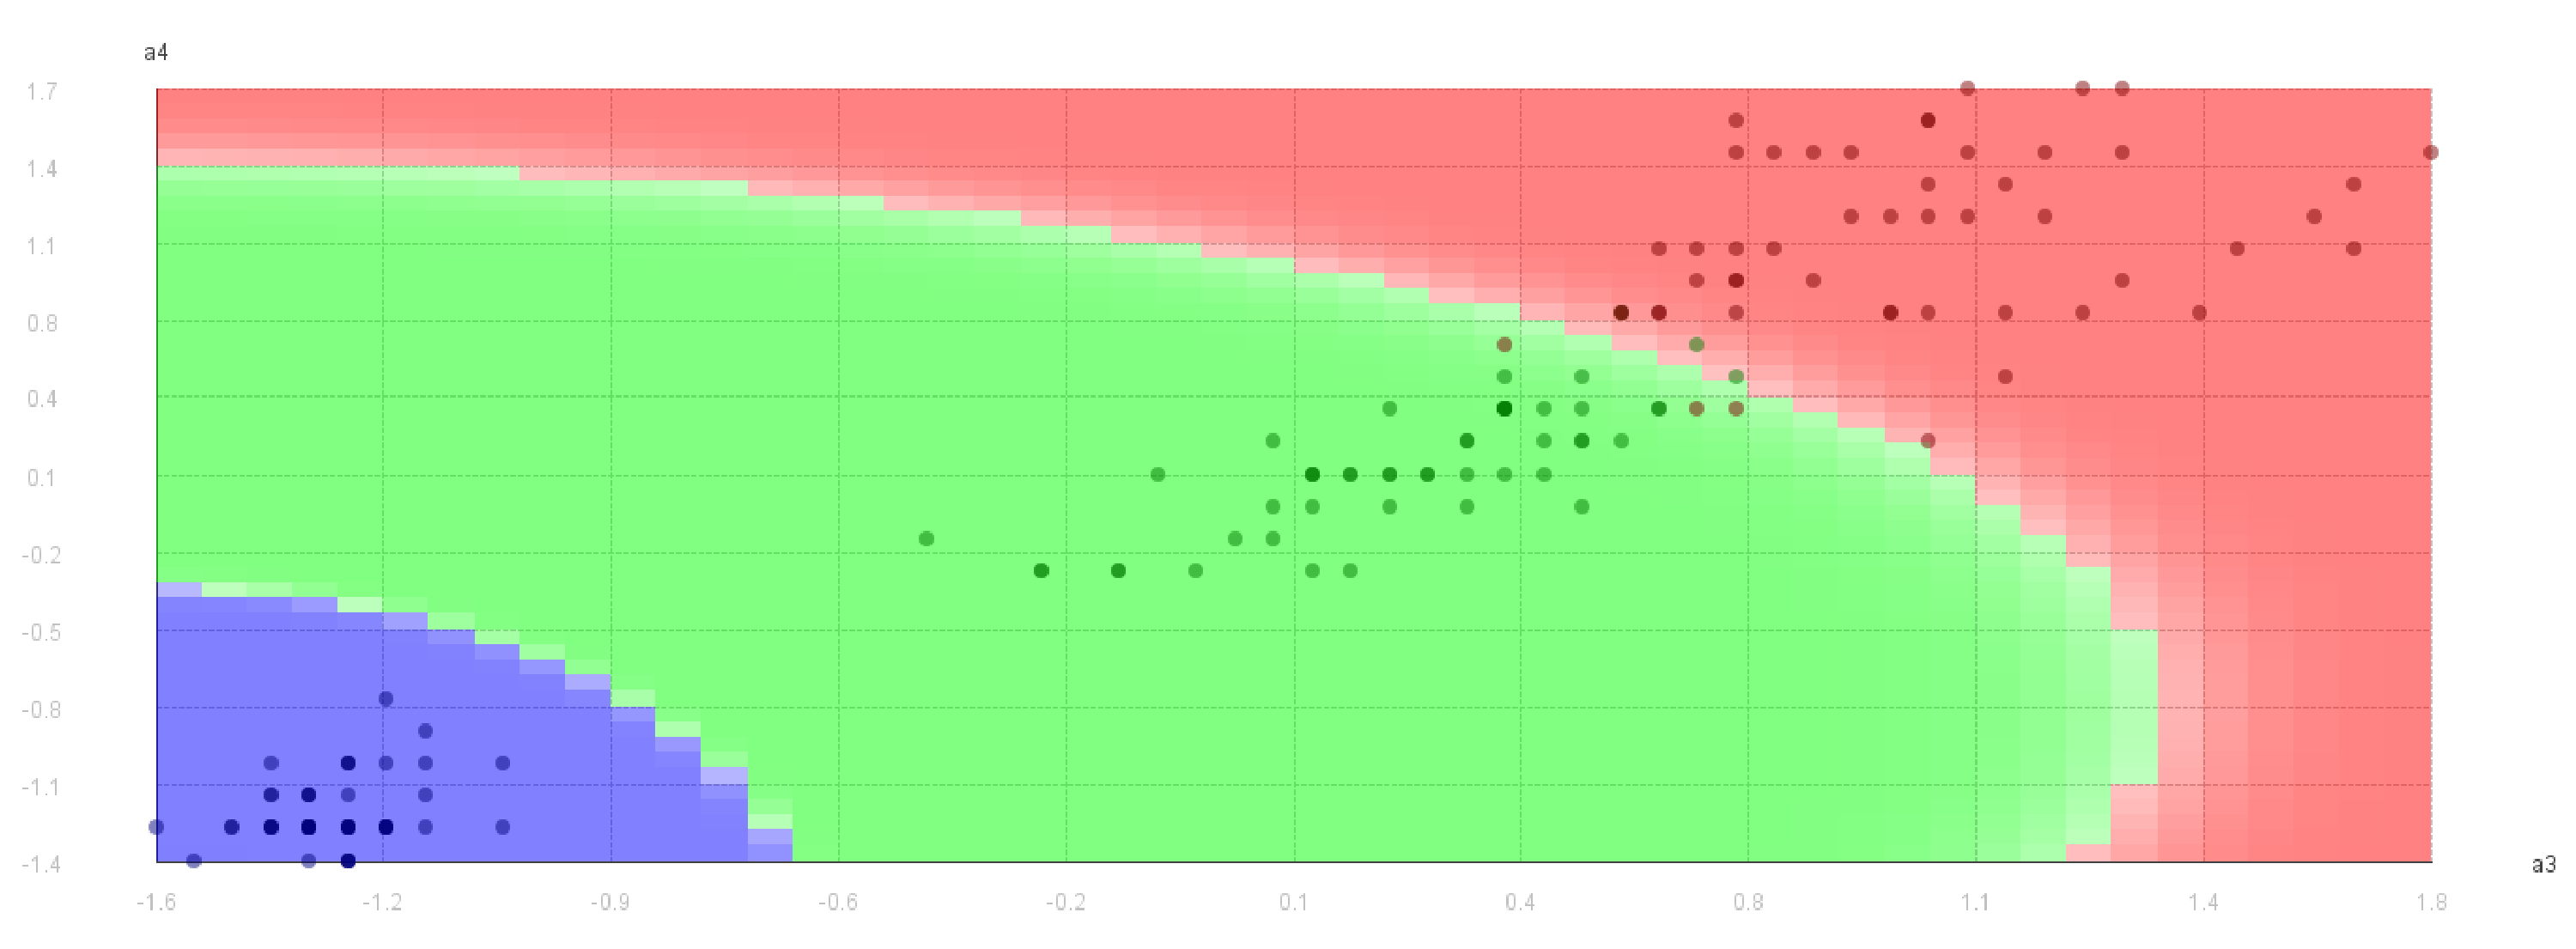
\includegraphics[width=0.98\textwidth,height=3.8cm,keepaspectratio]{images/slide19_decision_boundaries_clean.png}
  \end{center}
\end{frame}

% Slide 20: Naive Bayes Discussion
\begin{frame}{تحلیل و جمع‌بندی بیز ساده}{\lr{Naïve Bayes: Strengths \& Limitations}}
  \begin{itemize}
    \setlength{\itemsep}{7pt}
    \item \textbf{کارایی شگفت‌انگیز در عمل:} حتی با نقض آشکار فرض استقلال ویژگی‌ها، اغلب عملکرد عالی ارائه می‌دهد زیرا فقط رتبه نسبی درست‌نمایی برای تصمیم‌گیری مهم است.
    \item \textbf{مقاومت در برابر نویز} (\lr{Noise Robustness}): داده‌های پرت ایزوله اثر ناچیزی بر میانگین‌ها و توزیع کلی دارند.
    \item \textbf{مقاومت در برابر ویژگی‌های بی‌ارتباط} (\lr{Irrelevant Attributes}): زیرا این ویژگی‌ها توزیعی تقریباً یکنواخت برای تمامی کلاس‌ها خواهند داشت.
    \item \textbf{حساسیت به ویژگی‌های تکراری} (\lr{Redundant Attributes}): تکرار متغیرهای همبسته اثر یک ویژگی را مضاعف می‌کند (نیاز به انتخاب ویژگی).
    \item \textbf{مزایای فنی و محاسباتی بالا:}
    \begin{itemize}
      \item \textbf{زمان آموزش:} تنها با یک‌بار پیمایش داده‌ها (\lr{$O(Nd)$}).
      \item \textbf{حافظه مصرفی:} بسیار اندک جهت ذخیره‌سازی ماتریس احتمالات.
    \end{itemize}
  \end{itemize}
\end{frame}
